\documentclass[12pt]{article}

\usepackage[paperheight=8.5in,
            paperwidth=6.5in,
            margin=0.6in]{geometry}

\usepackage{avant, enumitem, graphicx, tikz, wrapfig, hyperref}
\renewcommand{\familydefault}{\sfdefault}
\setcounter{secnumdepth}{0}

\begin{document}

\tikz[remember picture,overlay] \node[inner sep=0pt] at (current page.center){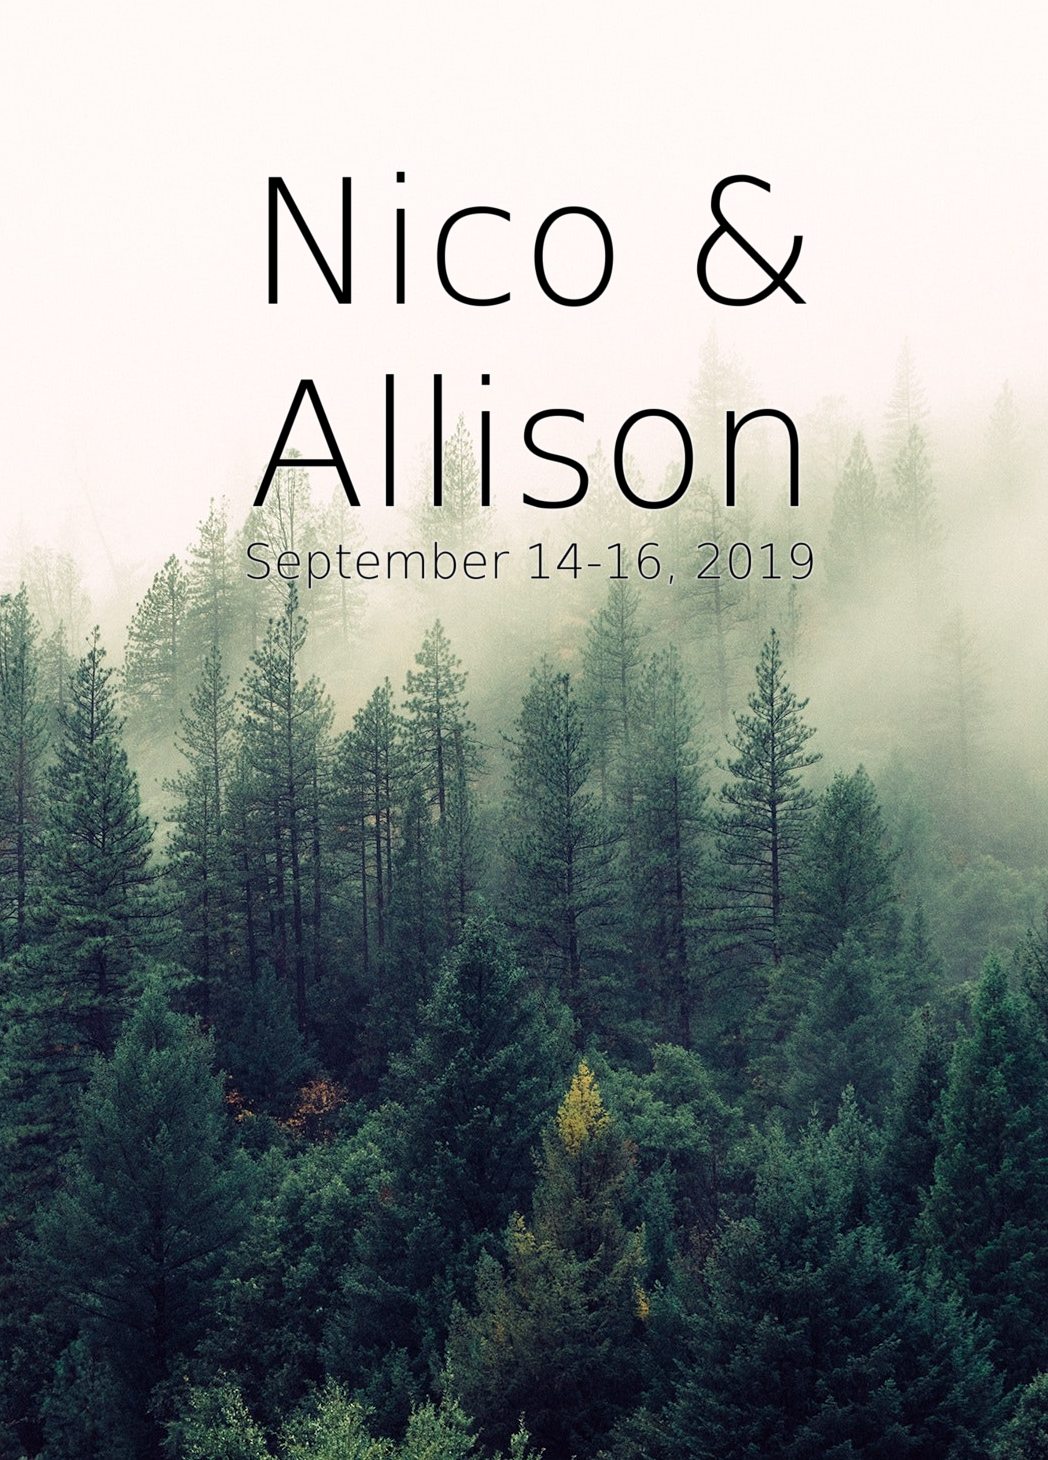
\includegraphics[width=\paperwidth,height=\paperheight]{cover}};
\pagenumbering{gobble}
\clearpage
\newpage

\begin{center}
    \Large Allison and Nico's Seattle Celebration!
\end{center}
\pagenumbering{arabic}
Thank you so much for coming out to see us and to celebrate our marriage!
We are so blessed to have such a loving and supportive family and we're excited to 
get to spend some quality time with you over the next couple of days!

\section{Events}
We have set up a series of events that you can choose to attend if you
are feeling up for it, but we also want you to feel free to explore our
wonderful city by yourself and ``choose your own adventure,'' if you feel so inclined.

To that effect, we have set up a loose schedule for this weekend that you should 
feel free to follow as closely as you desire! All of the following events
(besides the wedding celebration dinner Monday night) are completely optional! We will be there
and you're sure to run into some other friendly faces as well.

\begin{itemize}[leftmargin=0.25em]
    \item \textbf{Saturday, September 14}
    \begin{itemize}[leftmargin=1em]
        \item Most people will be arriving this day! Feel free to hit up the Pike Place market or 
        any of the other ideas we have on page~\pageref{sec-things-to-do}.
        \item \textbf{7pm} -- Drinks and bites at Peddler Brewing. See page~\pageref{subsec-dinner-sat} for details.
    \end{itemize}
    \item \textbf{Sunday, September 15}
    \begin{itemize}[leftmargin=1em]
        \item \textbf{10am-12pm} -- Hike in Discovery Park (page~\pageref{subsec-discovery})
        \item \textbf{12pm-2(ish)} -- Lunch/games in Discovery Park (page~\pageref{subsec-discovery})
        \item \textbf{7pm} -- Dinner at Rhein Haus (page~\pageref{subsec-rheinhaus})
    \end{itemize}
    \item \textbf{Monday, September 16}
    \begin{itemize}[leftmargin=1em]
        \item \textbf{9am} -- Yoga alongside Allison (page~\pageref{subsec-yoga})
        \item \textbf{6pm} -- Our wedding celebration dinner! (page~\pageref{subsec-wedding})
    \end{itemize}
\end{itemize}

%And that's it! If you are looking for more things to do, you can check out our favorite 
%places to eat, relax, and explore in this awesome city! Flip to page~\pageref{sec-things-to-do} for that.



\tableofcontents

\newpage

\vspace{0.5in}
\begin{figure}[h]
    \centering
    
\includegraphics[width=\textwidth]{logo-navy-80}
\end{figure}

\newpage

\section{Saturday Event Details}
Here you can read a bit more about the things we've planned to see which of them tickle your fancy.

\subsection{Meetup at Peddler Brewing}
\label{subsec-dinner-sat}
\begin{center}
    \texttt{1514 NW Leary Way, Seattle, WA 98107\\\href{Peddlerbrewing.com}{Peddlerbrewing.com}}
\end{center}

    Come on down and hang out with us at this family-friendly brew pub. We'll have a couple tables 
    in their covered outdoor area. Feel free to make a quick stop or hang out and play some of the 
    lawn and board games they offer. They have a food truck out back, a sandwich shop with a window 
    that has access to the brewery and they also allow you to bring your own food if you want to make 
    this your dinner stop for the evening. 


        \begin{center}
            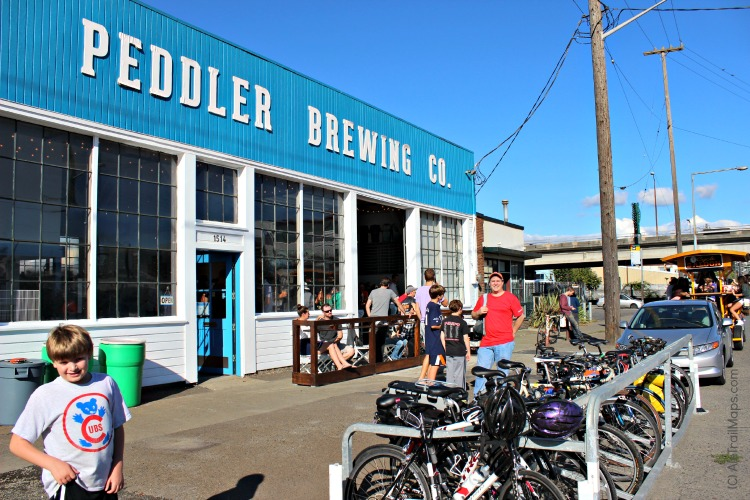
\includegraphics[width=0.8\textwidth]{peddler}
        \end{center}
    
    See page~\pageref{subsec-bites} for other places we like to grab grub! 



\newpage
\section{Sunday Event Details}
\subsection{Discovery Park Hike and Picnic Lunch}
This is one of Nico's absolute favorite spaces in the city. When he first arrived he was amazed 
by all the huge green spaces all around us and made it his quest to visit them all. The placement of 
this park played no small role in our decision to move to Magnolia. Now we live right next door and Nico gets to go running in the park
before school!\hfill
\label{subsec-discovery}

Discovery is the largest park in the city of Seattle. It clocks in at  
\begin{wrapfigure}{r}{0.5\textwidth}
    \begin{center}
        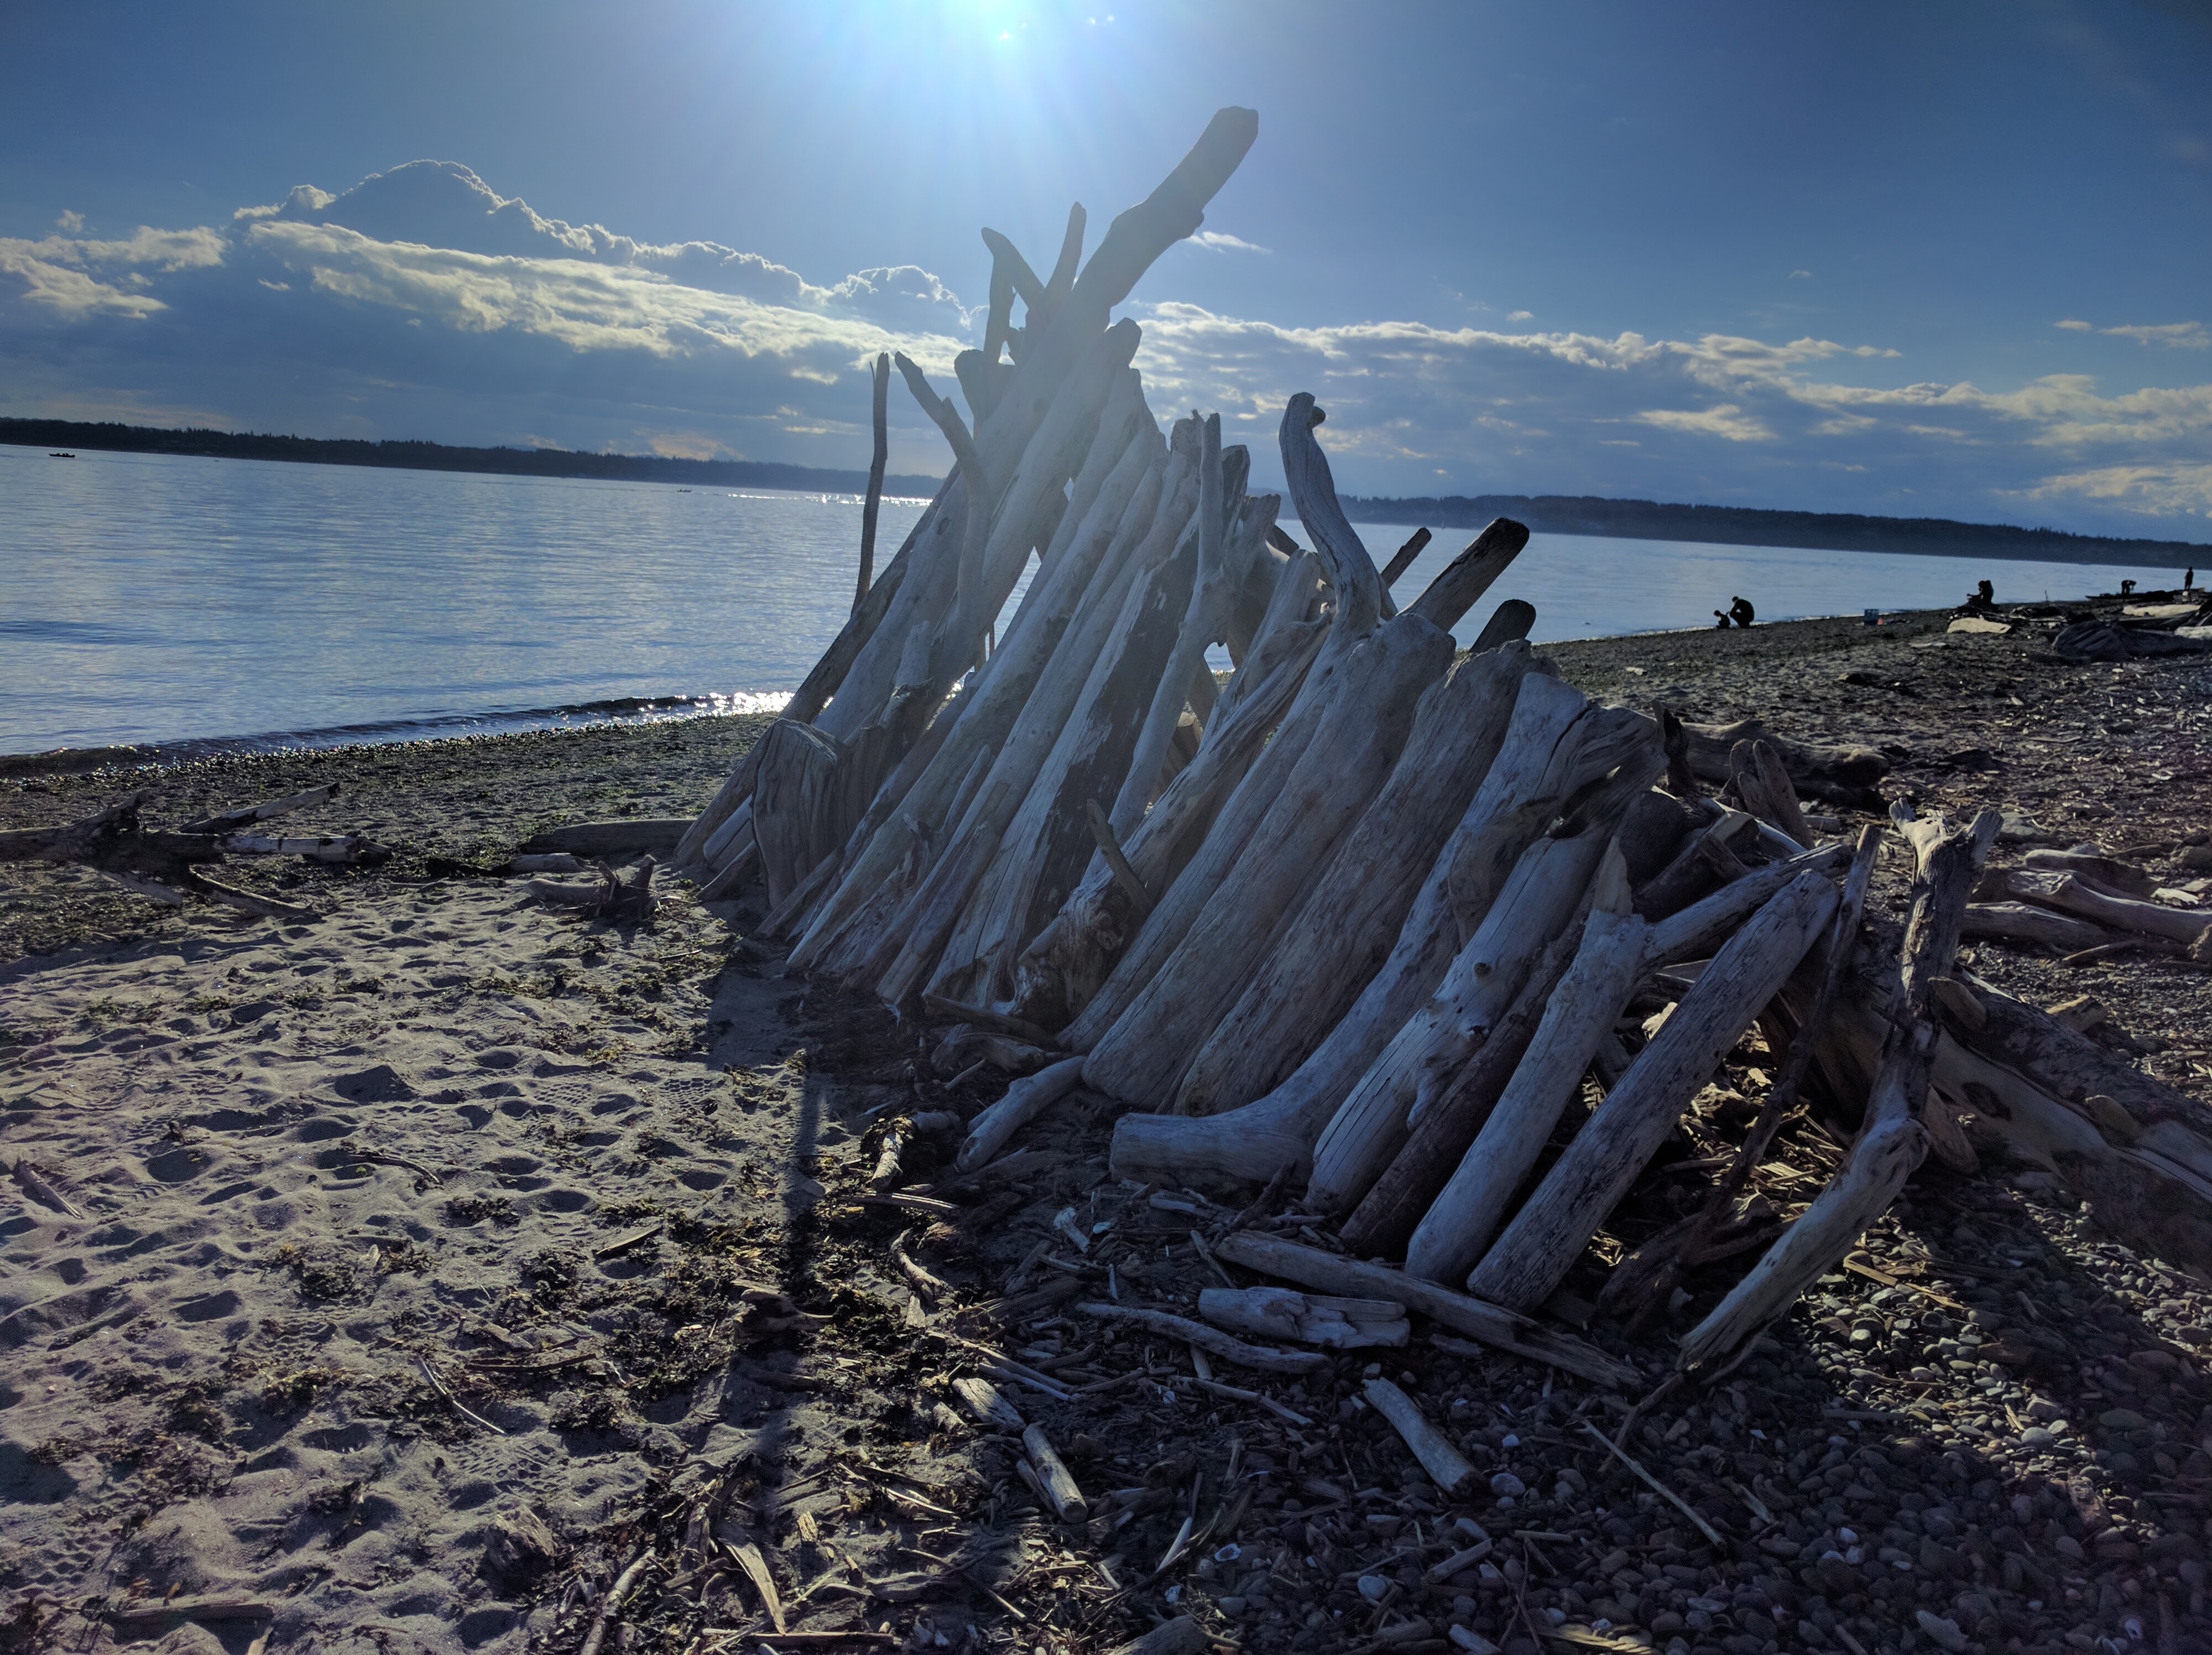
\includegraphics[width=0.48\textwidth]{leanto}
    \end{center}
\end{wrapfigure}
534 acres and it captures
a huge variety of different biomes. You can get (truly) lost among the trees in the vast
forested areas or stroll through a meadow to come to stunning bluffs overlooking Puget sound.

You can meet us at \textbf{10~am} on Sunday for a brisk walk through the forest and along the cliffs
to a cozy beach with a lighthouse and back. It's about 5mi round trip and there are about 400' of stairs
to climb but we won't be pushing too hard so hopefully anyone can join. If you'd prefer to skip it, you are 
still welcome to join us at noon for some food in the park (which will be hosted by Jeff and Colleen).

\textsc{If you are planning on going on the hike:} Just search for \textbf{Discovery Park East Parking Lot} in your favorite maps app and you will be led right there. For those of you
staying in Ballard, you can even try walking across the locks if you're looking for an extra bit of exercise. We love heading
down that path (in the opposite direction) for Sunday brunch. :)

\textsc{If you plan on meeting up with us after the hike:} We will have a picnic lunch provided by the Courts family 
on the bluffs overlooking Puget sound. This will be an old-fashioned ``blankets and baskets'' style picnic, set your GPS 
to \textbf{Discovery Park South Parking Lot} off W Emerson Drive. There will be a short walk from the lot to the bluffs, 
close to the ``Chapel-Ft Lawton Historical District'' that you'll also see on your maps app.

\subsection{Rhein Haus}
\label{subsec-rheinhaus}
\begin{center}
    \texttt{912 12th Ave, Seattle, WA 98122\\\href{https://www.rheinhausseattle.com/}{RheinHausSeattle.com}}
\end{center}

\textit{Of particular interest to our out-of-town guests:} Join us for a no-host buffet dinner at Rhein Haus in Capitol Hill. This fun and vibrant place combines Nico's 
adoration for all things German and Allison’s other true love: pretzels. We have a special section just for us 
and will have several delicious options to satisfy both the vegans and the carnivores among us! 

Due to the size 
of our group, we need to schedule many things 
\begin{wrapfigure}{l}{0.5\textwidth}
    \begin{center}
        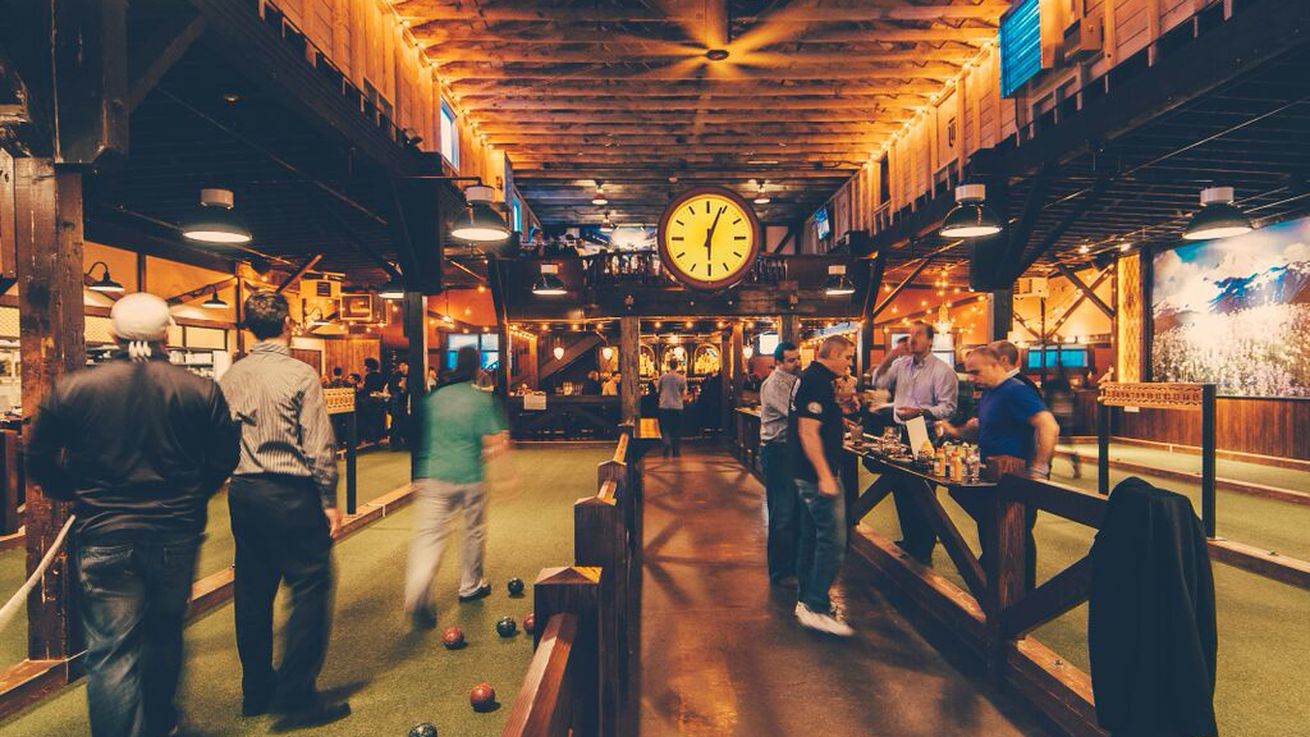
\includegraphics[width=0.48\textwidth]{rheinhaus}
    \end{center}
\end{wrapfigure}
ahead, so if you are coming please both RSVP (at \href{https://courtay.info}{our wedding website}) and bring cash/venmo 
\$20 per person to Nico (@Nicolas-Courts) or Allison (@AllisonStaciaTaylor) for food. Drinks are plentiful and up 
to you! Rhein Haus has over 20 drafts and lots o'bottles to choose from, not to mention options for bocce or other 
games throughout the establishment. 

We have the space from 6pm-8pm, feel free to come 
anytime during those hours---minors do need to be out of the property by 9pm.


\section{Monday Event Details}
\subsection{Yoga with Allison @ Shakti Yoga Seattle}
\label{subsec-yoga}
\begin{center}
    \texttt{2238 NW Market St, Seattle, WA 98107\\\href{http://shaktivinyasa.com/}{ShaktiVinyasa.com}}
\end{center}

Join Allison for an invigorating hot yoga session at 9:30am at her favorite studio. Arrive early to complete 
registration and rent a mat, you can also reserve your space in advance at 
\begin{center}
    \href{http://shaktivinyasa.com/seattle-schedule}{http://shaktivinyasa.com/seattle-schedule}.
\end{center}

Please note that Allison is not teaching this class, just taking it along with anyone else who wants to 
join in on the sweat!

\subsection{Wedding Celebration!}
\label{subsec-wedding}
Finally the main event! Join us in downtown Ballard at the \textbf{Olympic Rooftop Pavillion} at
the \textbf{Hotel Ballard} at \textbf{6pm}.
\begin{center}
    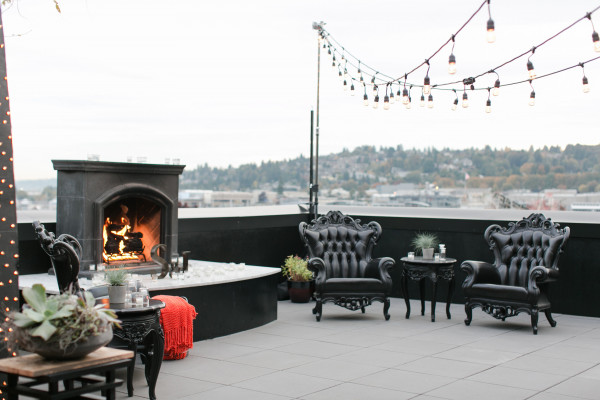
\includegraphics[width=0.48\textwidth]{pavillion}
\end{center}

We will begin with some time with appetizers and cocktails and time for us all to socialize in this beautiful event space at the top of the Ballard skyline.
Dinner will follow and will be some delicious food served family-style with something for vegetarians and meat eaters alike. Catering will 
be by the great Stoneburner restaurant downstairs (a local favorite).

\newpage
\section{Things to Do and See in Seattle}
\label{sec-things-to-do}
We've pulled together our combined recommendations for things to do, see, and eat.
Hopefully these things float your boat!
\renewcommand\thesubsubsection{\arabic{subsubsection}}

\noindent\hrulefill

\subsection{Touristy Stuff}
What kind of city guide would this be if we didn't include the stuff that tourists like 
to do? If you ask a Seattlite, they'd never be caught dead in these places although secretly
we've all been to most of these places at least once.

You can find everything on the map below with the numbers corresponding to the number in each heading.

\subsubsection{Pike Place Market}
Don't you dare call it ``\textit{Pike's} place''! This is a bustling market 
\begin{wrapfigure}{r}{0.5\textwidth}
    \centering
    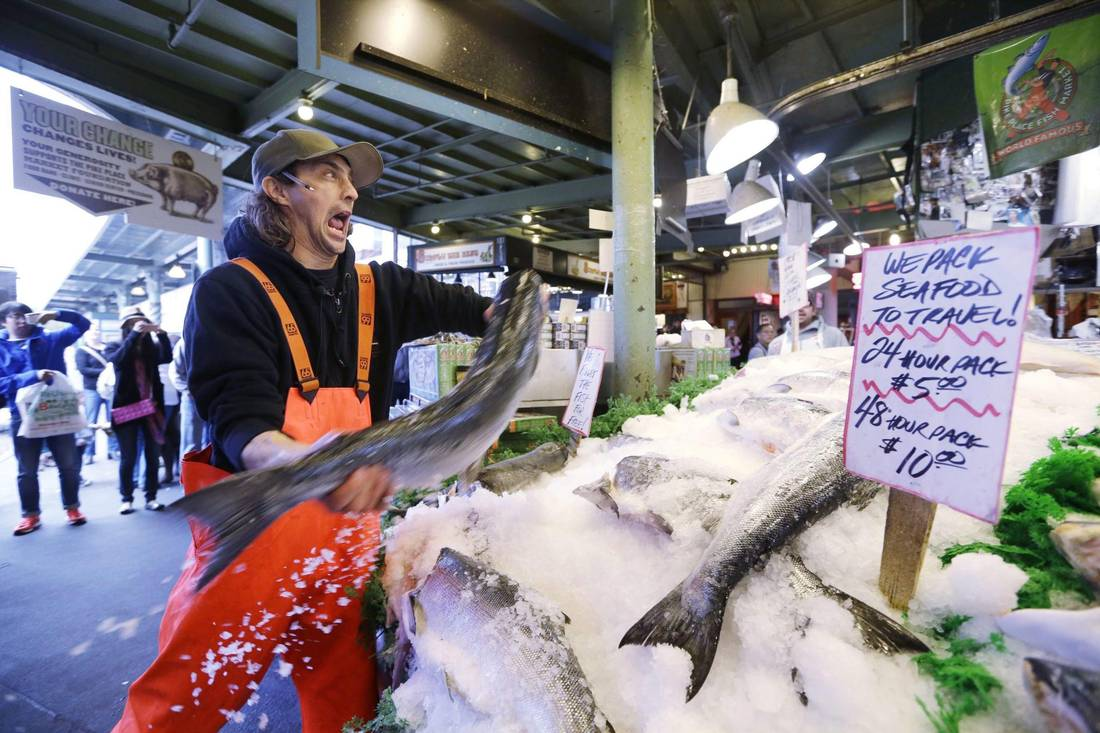
\includegraphics[width=0.48\textwidth]{fish.jpg}
\end{wrapfigure}
right in the middle
of downtown that is famous for, among other things, the fishmongers who throw their fresh
fish back and forth. We love it for the fantastic deals you can get on fresh bouquets and the
cute hand-crafted goods you can find there.

If you're feeling nostalgic (and you have too much time on your hands) you can also visit the first Starbucks
which is located right across the street. We'd recommend walking about 500 feet down the street
and getting the \textit{exact same cup of coffee} from a more modern Starbucks with a fraction of the wait, however. :)

\subsubsection{Smith Tower}
Sure, you \textit{could} go to the space needle but honestly we've gone there and paid the \$40 fee to ride up in
the elevator and it's a bit of a bust. And this is on top of having to pay for parking and navigate the craziness
of downtown.

Instead, let us offer you the Smith Tower as an alternative. Have you ever wanted to feel like you 
were part of the 1920s upper crust? Well you're in luck because for the low, low price of \$20 you 
can get 
\begin{wrapfigure}{l}{0.5\textwidth}
    \centering
    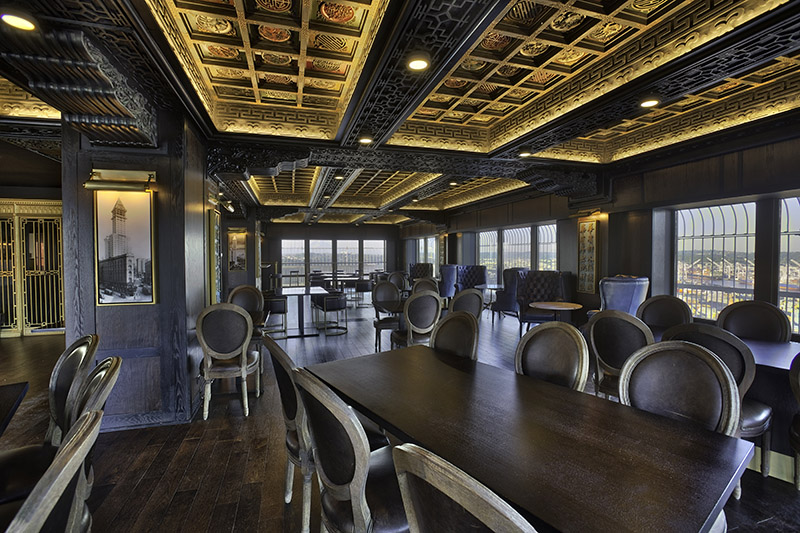
\includegraphics[width=0.48\textwidth]{smith.jpg}
\end{wrapfigure}
a historical tour of the building followed by a ride up in the elevator to the Observatory Bar,
a luxurious room with 360 degree views of Seattle and the Sound and one thing that you'll 
never see from the Space Needle: the Space Needle itself!

Allison absolutely fell in love with the tower when she first visited when she was younger
and has since convinced Nico to love it (almost) as much.

You can also choose to visit after hours (after 9pm) to shave \$8 off the admission price.

\noindent\hrulefill

\subsection{Bites to Eat}
\label{subsec-bites}

\subsubsection{\textit{Perch\'e No}}
\begin{center}
    \texttt{1319 N 49th St Seattle, WA, 98103}
\end{center}
This wonderful restaurant is where Allison and Nico had one of their very first dates!
It is an Italian restaurant owned and run by a Korean couple -- he is the head chef and 
she works the front of the house -- and it's to die for. 

It has a fun ambiance and the whole restaurant surrounds a big open kitchen where you can 
watch the chef boil up your fresh house-made pasta and enjoy a glass of wine from their 
extensive wine list. On our first trip the owner came up to us and told us all about her son 
who just started a food truck -- she was so proud!

\subsubsection{\textit{Mondello Ristorante Italiano}}
\begin{center}
    \texttt{2425 33rd Ave W \#3 Seattle, WA 98199}
\end{center}
Speaking of incredible Italian food, \textit{Mondello} is our new secret spot (shhh...) 
to take people from out of town. Come inside and you are in your family's kitchen (or 
maybe some idealized version that cleans up) and a sweet Sicilian lady will come up and
treat you like one of her own. The food is authentic with a capital ``A'' and you'll 
swear that you have been magically transported to the south of Italy.

For an added bonus, you can pop next door for some Gelato from the Nutty Squirrel! They 
have gelato and sorbetto for the vegans among you.

\subsubsection{Pink Salt}
\begin{center}
    \texttt{3321 W. McGraw St Seattle, WA 98199\\\href{https://pinksaltseattle.com/}{PinkSaltSeattle.com}}
\end{center}
The owners of \textit{Mondello} bought another space right down the street and decided to create 
their own version of Peruvian cuisine! Worth a visit if only to see the glowing wall behind the bar
entirely made of pink salt (Nico tasted it for authenticity)! The cocktails are innovative and delicious 
and the food made us both happy.

\subsubsection{Pel'Meni Dumpling Tzar}
\begin{center}
    \texttt{1630 12th Ave, Seattle, WA 98122\\\href{http://dumplingtzar.com/}{DumplingTzar.com}}
\end{center}
This place is a surprise-- inexpensive dumplings with delicious choices for toppings and a pretty 
great bar, too. Allison quickly fell in love with this place (definitely visit the Capitol Hill location 
listed here for a fuller menu vs the Fremont one) and discovered Vareniki fries. 
\begin{center}
    \textit{You're welcome in advance.}    
\end{center}
\hrulefill

\subsection{The Caf\'e Life}
\label{subsec-cafe}
Seattle is definitely known for its coffee scene, but these caf\'es have stood out to us as truly outstanding.
\subsubsection{Miro Tea}
\begin{center}
    \texttt{5405 Ballard Ave NW, Seattle, WA 98107\\\href{http://mirotea.com/}{MiroTea.com}}
\end{center}

Okay, so it's not coffee. But if you are a tea drinker like Nico you will almost certainly
find something you love. They have some outstanding Chinese tea (Nico always gets a \textit{gaiwan} of \textit{puerh} tea)
and some friendly staff who know what they're talking about.

The best part is that, if you're staying in Ballard, it's right around the corner!

\subsubsection{La Marzocco}
\begin{center}
    \texttt{472 1st Ave N, Seattle, WA 98109 \\\href{https://lamarzoccousa.com}{LaMarzoccoUsa.com}}
\end{center}
The showroom for La Marzocco espresso machines, this shop hosts a rotating cast of coffee roasters and 
the menu changes monthly. The space is shared with Seattle's local-powered KEXP radio station and comes 
complete with a Molly Moon's ice cream machine (a local delicacy). 

\subsubsection{Storyville Coffee}
\begin{center}
    \texttt{Found at Pike Place and in Queen Anne\\\href{https://storyville.com/}{Storyville.com}}
\end{center}
Allison's favorite coffee place, they have homemade baked goods, delicious roasts, and the absolute best logo.

\subsubsection{Milstead Coffee}
\begin{center}
    \texttt{54 N 34th St, Seattle, WA 98103\\\href{http://milsteadandco.com/}{MilsteadAndCo.com}}
\end{center}
Dang good coffee right by one of the crew boathouses Allison (and her dad) rows out of on Lake Union. 
Walk up Troll Ave to see the famous Seattle troll featured in the 1999 masterpiece \textit{10 Things I Hate About You}.

\subsubsection{Espresso Vivace}
\begin{center}
    \texttt{Several Locations\\\href{http://espressovivace.com/}{Espresso Vivace}}
\end{center}
You MUST try the Cafe Nico drink on their menu. First tasted because of the name, this is the speciality of 
the house and easily one of the top 5 coffee drinks you’ll ever have in your life.

\noindent\hrulefill 

\subsection{Bars and Nightlife}
Looking to shake your groove thing or get your drank on? Luckily there are some happening
spots for you hep cats.
\subsubsection{Pie Bar Ballard}
\begin{center}
    \texttt{2218 NW Market St, Seattle, WA 98107}
\end{center}

As you probably know, Allison can't have gluten and Nico doesn't drink. Luckily that isn't a problem 
for them because Pie Bar is a thing! Right down the street from the Ballard Hotel sits this warm
little shop with a cozy ambiance where you can go alone or with a group to go grab a slice and/or a cocktail.

People are friendly and the pie is great and you'd be hard pressed to have a bad time here.

\subsubsection{Garage Capitol Hill}

\subsubsection{Deep Dive}
\begin{center}
    \texttt{a}
\end{center}

\subsubsection{Bitterroot BBQ}

\subsubsection{The Noble Fir}


\end{document}